\documentclass{beamer}
\usepackage{amsmath,graphics}
\usepackage{amssymb}

\usetheme{default}
\usepackage{xcolor}

\definecolor{solarizedBase03}{HTML}{002B36}
\definecolor{solarizedBase02}{HTML}{073642}
\definecolor{solarizedBase01}{HTML}{586e75}
\definecolor{solarizedBase00}{HTML}{657b83}
\definecolor{solarizedBase0}{HTML}{839496}
\definecolor{solarizedBase1}{HTML}{93a1a1}
\definecolor{solarizedBase2}{HTML}{EEE8D5}
\definecolor{solarizedBase3}{HTML}{FDF6E3}
\definecolor{solarizedYellow}{HTML}{B58900}
\definecolor{solarizedOrange}{HTML}{CB4B16}
\definecolor{solarizedRed}{HTML}{DC322F}
\definecolor{solarizedMagenta}{HTML}{D33682}
\definecolor{solarizedViolet}{HTML}{6C71C4}
%\definecolor{solarizedBlue}{HTML}{268BD2}
\definecolor{solarizedBlue}{HTML}{134676}
\definecolor{solarizedCyan}{HTML}{2AA198}
\definecolor{solarizedGreen}{HTML}{859900}
\definecolor{myBlue}{HTML}{162DB0}%{261CA4}
\setbeamercolor*{item}{fg=myBlue}
\setbeamercolor{normal text}{fg=solarizedBase03, bg=solarizedBase3}
\setbeamercolor{alerted text}{fg=myBlue}
\setbeamercolor{example text}{fg=myBlue, bg=solarizedBase3}
\setbeamercolor*{frametitle}{fg=solarizedRed}
\setbeamercolor*{title}{fg=solarizedRed}
\setbeamercolor{block title}{fg=myBlue, bg=solarizedBase3}
\setbeameroption{hide notes}
\setbeamertemplate{note page}[plain]
\beamertemplatenavigationsymbolsempty
\usefonttheme{professionalfonts}
\usefonttheme{serif}

\usepackage{fourier}

\def\vec#1{\mathchoice{\mbox{\boldmath$\displaystyle#1$}}
{\mbox{\boldmath$\textstyle#1$}}
{\mbox{\boldmath$\scriptstyle#1$}}
{\mbox{\boldmath$\scriptscriptstyle#1$}}}
\definecolor{OwnGrey}{rgb}{0.560,0.000,0.000} % #999999
\definecolor{OwnBlue}{rgb}{0.121,0.398,0.711} % #1f64b0
\definecolor{red4}{rgb}{0.5,0,0}
\definecolor{blue4}{rgb}{0,0,0.5}
\definecolor{Blue}{rgb}{0,0,0.66}
\definecolor{LightBlue}{rgb}{0.9,0.9,1}
\definecolor{Green}{rgb}{0,0.5,0}
\definecolor{LightGreen}{rgb}{0.9,1,0.9}
\definecolor{Red}{rgb}{0.9,0,0}
\definecolor{LightRed}{rgb}{1,0.9,0.9}
\definecolor{White}{gray}{1}
\definecolor{Black}{gray}{0}
\definecolor{LightGray}{gray}{0.8}
\definecolor{Orange}{rgb}{0.1,0.2,1}
\setbeamerfont{sidebar right}{size=\scriptsize}
\setbeamercolor{sidebar right}{fg=Black}

\renewcommand{\emph}[1]{{\textcolor{solarizedRed}{\itshape #1}}}

\newcommand\dd{\mathrm d}

\newcommand\cA{\mathcal A}
\newcommand\cB{\mathcal B}
\newcommand\cC{\mathcal C}
\newcommand\cD{\mathcal D}
\newcommand\cE{\mathcal E}
\newcommand\cF{\mathcal F}
\newcommand\cG{\mathcal G}
\newcommand\cH{\mathcal H}
\newcommand\cI{\mathcal I}
\newcommand\cJ{\mathcal J}
\newcommand\cK{\mathcal K}
\newcommand\cL{\mathcal L}
\newcommand\cM{\mathcal M}
\newcommand\cN{\mathcal N}
\newcommand\cO{\mathcal O}
\newcommand\cP{\mathcal P}
\newcommand\cQ{\mathcal Q}
\newcommand\cR{\mathcal R}
\newcommand\cS{\mathcal S}
\newcommand\cT{\mathcal T}
\newcommand\cU{\mathcal U}
\newcommand\cV{\mathcal V}
\newcommand\cW{\mathcal W}
\newcommand\cX{\mathcal X}
\newcommand\cY{\mathcal Y}
\newcommand\cZ{\mathcal Z}

\newcommand\fA{\mathfrak A}
\newcommand\fB{\mathfrak B}
\newcommand\fC{\mathfrak C}
\newcommand\fD{\mathfrak D}
\newcommand\fE{\mathfrak E}
\newcommand\fF{\mathfrak F}
\newcommand\fG{\mathfrak G}
\newcommand\fH{\mathfrak H}
\newcommand\fI{\mathfrak I}
\newcommand\fJ{\mathfrak J}
\newcommand\fK{\mathfrak K}
\newcommand\fL{\mathfrak L}
\newcommand\fM{\mathfrak M}
\newcommand\fN{\mathfrak N}
\newcommand\fO{\mathfrak O}
\newcommand\fP{\mathfrak P}
\newcommand\fQ{\mathfrak Q}
\newcommand\fR{\mathfrak R}
\newcommand\fS{\mathfrak S}
\newcommand\fT{\mathfrak T}
\newcommand\fU{\mathfrak U}
\newcommand\fV{\mathfrak V}
\newcommand\fW{\mathfrak W}
\newcommand\fX{\mathfrak X}
\newcommand\fY{\mathfrak Y}
\newcommand\fZ{\mathfrak Z}

\newcommand\fa{\mathfrak a}
\newcommand\fb{\mathfrak b}
\newcommand\fc{\mathfrak c}
\newcommand\fd{\mathfrak d}
\newcommand\fe{\mathfrak e}
\newcommand\ff{\mathfrak f}
\newcommand\fg{\mathfrak g}
\newcommand\fh{\mathfrak h}
%\newcommand\fi{\mathfrak i}
\newcommand\fj{\mathfrak j}
\newcommand\fk{\mathfrak k}
\newcommand\fl{\mathfrak l}
\newcommand\fm{\mathfrak m}
\newcommand\fn{\mathfrak n}
\newcommand\fo{\mathfrak o}
\newcommand\fp{\mathfrak p}
\newcommand\fq{\mathfrak q}
\newcommand\fr{\mathfrak r}
\newcommand\fs{\mathfrak s}
\newcommand\ft{\mathfrak t}
\newcommand\fu{\mathfrak u}
\newcommand\fv{\mathfrak v}
\newcommand\fw{\mathfrak w}
\newcommand\fx{\mathfrak x}
\newcommand\fy{\mathfrak y}
\newcommand\fz{\mathfrak z}

\newcommand\vA{\vec A}
\newcommand\vB{\vec B}
\newcommand\vC{\vec C}
\newcommand\vD{\vec D}
\newcommand\vE{\vec E}
\newcommand\vF{\vec F}
\newcommand\vG{\vec G}
\newcommand\vH{\vec H}
\newcommand\vI{\vec I}
\newcommand\vJ{\vec J}
\newcommand\vK{\vec K}
\newcommand\vL{\vec L}
\newcommand\vM{\vec M}
\newcommand\vN{\vec N}
\newcommand\vO{\vec O}
\newcommand\vP{\vec P}
\newcommand\vQ{\vec Q}
\newcommand\vR{\vec R}
\newcommand\vS{\vec S}
\newcommand\vT{\vec T}
\newcommand\vU{\vec U}
\newcommand\vV{\vec V}
\newcommand\vW{\vec W}
\newcommand\vX{\vec X}
\newcommand\vY{\vec Y}
\newcommand\vZ{\vec Z}

\newcommand\va{\vec a}
\newcommand\vb{\vec b}
\newcommand\vc{\vec c}
\newcommand\vd{\vec d}
\newcommand\ve{\vec e}
\newcommand\vf{\vec f}
\newcommand\vg{\vec g}
\newcommand\vh{\vec h}
\newcommand\vi{\vec i}
\newcommand\vj{\vec j}
\newcommand\vk{\vec k}
\newcommand\vl{\vec l}
\newcommand\vm{\vec m}
\newcommand\vn{\vec n}
\newcommand\vo{\vec o}
\newcommand\vp{\vec p}
\newcommand\vq{\vec q}
\newcommand\vr{\vec r}
\newcommand\vs{\vec s}
\newcommand\vt{\vec t}
\newcommand\vu{\vec u}
\newcommand\vv{\vec v}
\newcommand\vw{\vec w}
\newcommand\vx{\vec x}
\newcommand\vy{\vec y}
\newcommand\vz{\vec z}

\renewcommand\AA{\mathbb A}
\newcommand\NN{\mathbb N}
\newcommand\ZZ{\mathbb Z}
\newcommand\PP{\mathbb P}
\newcommand\QQ{\mathbb Q}
\newcommand\RR{\mathbb R}
\newcommand\RRpos{\mathbb R_{\geq0}}
\renewcommand\SS{\mathbb S}
\newcommand\CC{\mathbb C}

\newcommand{\ord}{\mathrm{ord}}
\newcommand{\id}{\mathrm{id}}
\newcommand{\pr}{\mathrm{P}}
\newcommand{\Vol}{\mathrm{vol}}
\newcommand\norm[1]{\left\|{#1}\right\|} 
\newcommand\sign{\mathrm{sign}}
\newcommand{\eps}{\varepsilon}
\newcommand{\abs}[1]{\left|#1\right|}
\newcommand\bc[1]{\left({#1}\right)} 
\newcommand\cbc[1]{\left\{{#1}\right\}} 
\newcommand\bcfr[2]{\bc{\frac{#1}{#2}}} 
\newcommand{\bck}[1]{\left\langle{#1}\right\rangle} 
\newcommand\brk[1]{\left\lbrack{#1}\right\rbrack} 
\newcommand\scal[2]{\bck{{#1},{#2}}} 
\newcommand{\vecone}{\mathbb{1}}
\newcommand{\tensor}{\otimes}
\newcommand{\diag}{\mathrm{diag}}
\newcommand{\ggt}{\mathrm{ggT}}
\newcommand{\kgv}{\mathrm{kgV}}
\newcommand{\trans}{\top}

\newcommand{\Karonski}{Karo\'nski}
\newcommand{\Erdos}{Erd\H{o}s}
\newcommand{\Renyi}{R\'enyi}
\newcommand{\Lovasz}{Lov\'asz}
\newcommand{\Juhasz}{Juh\'asz}
\newcommand{\Bollobas}{Bollob\'as}
\newcommand{\Furedi}{F\"uredi}
\newcommand{\Komlos}{Koml\'os}
\newcommand{\Luczak}{\L uczak}
\newcommand{\Kucera}{Ku\v{c}era}
\newcommand{\Szemeredi}{Szemer\'edi}

\renewcommand{\ae}{\"a}
\renewcommand{\oe}{\"o}
\newcommand{\ue}{\"u}
\newcommand{\Ae}{\"A}
\newcommand{\Oe}{\"O}
\newcommand{\Ue}{\"U}

\newcommand{\im}{\mathrm{im}}
\newcommand{\rrk}{\mathrm{zrg}}
\newcommand{\crk}{\mathrm{srg}}
\newcommand{\rk}{\mathrm{rg}}
\newcommand{\GL}{\mathrm{GL}}
\newcommand{\SL}{\mathrm{SL}}
\newcommand{\SO}{\mathrm{SO}}
\newcommand{\nul}{\mathrm{nul}}
\newcommand{\eig}{\mathrm{eig}}

\newcommand{\mytitle}{Das Integral}

\title[Annuma]{\mytitle}
\author[Amin Coja-Oghlan]{Amin Coja-Oghlan}
\institute[Frankfurt]{JWGUFFM}
\date{}

\begin{document}

\frame[plain]{\titlepage}

\begin{frame}\frametitle{\mytitle}
	\begin{block}{Worum geht es?}
		\begin{itemize}
			\item Das Integral einer Funktion gibt die Fl\ae che an, die die Funktion mit der Abszisse einschlie\ss t.
			\item Anders ausgedr\ue ckt: wenn eine Funktion $f$ die Geschwindigkeit einer Bewegung angibt, erhalten wir durch das Integral die Position zu einem bestimmten Zeitpunkt.
			\item Wir lernen in dieser Vorlesung das Riemann-Integral kennen.
		\end{itemize}
	\end{block}
\end{frame}

\begin{frame}\frametitle{\mytitle}
\hfill	\includegraphics[height=20mm]{pics/int1.pdf}
	\begin{block}{Treppenfunktionen}
		\begin{itemize}
			\item Seien $a<b$ reelle Zahlen und sei $c\in\RR$ eine weitere Zahl.
			\item Die Funktion $f:[a,b]\to\RR,\ x\mapsto c$
				ist konstant.
			\item Die Fl\ae che, die sie mit der Abszisse einschlie\ss t, ist ein Rechteck.
			\item Wir definieren das Integral von $f$ als
				\begin{align*}
					\int_a^bf(x)\dd x=c(b-a).
				\end{align*}
			\item Je nach Vorzeichen von $c$ ist das Integral positiv oder negativ.
		\end{itemize}
	\end{block}
\end{frame}

\begin{frame}\frametitle{\mytitle}
\hfill	\includegraphics[height=20mm]{pics/int2.pdf}
	\begin{block}{Treppenfunktionen}
		\begin{itemize}
			\item Eine Funktion $f:[a,b]\to\RR$ hei\ss t eine \emph{Treppenfunktion}, wenn es Zahlen $\ell\in\NN$, $c_1,\ldots,c_\ell\in\RR$ und
				\begin{align*}
				a=s_0\leq\cdots\leq s_\ell=b
				\end{align*}
				gibt, so da\ss
				\begin{align*}
					f(x)=c_i\qquad\mbox{f\ue r alle }x,y\in(s_{i-1},s_{i}),\ i=1,\ldots,\ell.
				\end{align*}
			\item Mit anderen Worten: die Funktion ist auf den ``Treppenstufen'' $(s_{i-1},s_i)$ konstant.
		\end{itemize}
	\end{block}
\end{frame}

\begin{frame}\frametitle{\mytitle}
\hfill	\includegraphics[height=20mm]{pics/int2.pdf}
	\begin{block}{Treppenfunktionen}
		\begin{itemize}
	\item Das Integral einer Treppenfunktion ist definiert als
		\begin{align*}
			\int_a^b f(x)\dd x&=\sum_{i=1}^\ell c_i(s_i-s_{i-1}).
		\end{align*}
	\item Mit $\cT(a,b)$ bezeichnen wir die Menge aller Treppenfunktionen auf $[a,b]$.
		\end{itemize}
	\end{block}
\end{frame}

\begin{frame}\frametitle{\mytitle}
\hfill	\includegraphics[height=20mm]{pics/int3.pdf}
	\begin{block}{Riemannsche Obersummen}
		\begin{itemize}
			\item Sei $f:[a,b]\to\RR$ eine Funktion.
			\item Sei $g\in\cT(a,b)$ eine Treppenfunktion ist.
			\item Wir schreiben $f\leq g$, wenn
				\begin{align*}
					f(x)\leq g(x)\qquad\mbox{f\ue r alle }x\in[a,b],
				\end{align*}
			\item In diesem Fall nennen wir das Integral
				\begin{align*}
					\int_a^bg(x)\dd x
				\end{align*}
				eine \emph{Riemannsche Obersumme} von $f$.
		\end{itemize}
	\end{block}
\end{frame}

\begin{frame}\frametitle{\mytitle}
\hfill	\includegraphics[height=20mm]{pics/int4.pdf}
	\begin{block}{Riemannsche Untersummen}
		\begin{itemize}
			\item Wir schreiben $f\geq h\in\cT(a,b)$, wenn
				\begin{align*}
					f(x)\geq h(x)\qquad\mbox{f\ue r alle }x\in[a,b],
				\end{align*}
			\item In diesem Fall nennen wir das Integral
				\begin{align*}
					\int_a^bh(x)\dd x
				\end{align*}
				eine \emph{Riemannsche Untersumme} von $f$.
		\end{itemize}
	\end{block}
\end{frame}

\begin{frame}\frametitle{\mytitle}
	\begin{block}{Definition}
		Eine Funktion $f:[a,b]\to\RR$ hei\ss t \emph{integrabel}, wenn es Treppenfunktionen $g,h$ mit
		$ h\leq f\leq g $ gibt und
		\begin{align*}
			&\sup\cbc{\int_a^bh(x)\dd x:h\in\cT(a,b),\ h\leq f}\\&=\inf\cbc{\int_a^bg(x)\dd x:g\in\cT(a,b),\ g\geq f}.
		\end{align*}
		In diesem Fall definiern wir das \emph{Integral von $f$} als
		\begin{align*}
			\int_a^bf(x)\dd x=\sup\cbc{\int_a^bh(x)\dd x:h\in\cT(a,b),\ h\leq f}.
		\end{align*}
	\end{block}
\end{frame}

\begin{frame}\frametitle{\mytitle}
	\begin{block}{Satz}
		Jede Funktion $f:[a,b]\to\RR$, die
	\begin{itemize}
		\item stetig ist, oder
		\item monoton wachsend ist, oder
		\item monoton fallend ist, 
	\end{itemize}
	ist integrabel.
	\end{block}
\end{frame}

\begin{frame}\frametitle{\mytitle}
	\begin{block}{Proposition}
		Seien $f,g:[a,b]\to\RR$ integrabel und seien $s,t\in\RR$.
		Dann ist die Funktion
		\begin{align*}
			s\cdot f+t\cdot g:[a,b]\to\RR,\qquad x\mapsto s\cdot f(x)+t\cdot g(x)
		\end{align*}
		integrabel und
		\begin{align*}
			\int_a^b s\cdot f(x)+t\cdot g(x)\dd x=s\int_a^b f(x)\dd x+t\int_a^bg(x)\dd x.
		\end{align*}
	\end{block}
\end{frame}

\begin{frame}\frametitle{\mytitle}
	\begin{block}{Proposition}
		Seien $f,g:[a,b]\to\RR$ integrabel.
		Wenn $f\leq g$, dann gilt
		\begin{align*}
			\int_a^bf(x)\dd x\leq\int_a^bg(x)\dd x.
		\end{align*}
	\end{block}
\end{frame}

\begin{frame}\frametitle{\mytitle}
	\begin{block}{Proposition}
		Sei $f:[a,b]\to\RR$ integrabel und $c\in(a,b)$.
		Dann sind die Funktionen
		\begin{align*}
			[a,c]\to\RR,\qquad x\mapsto f(x)\\
			[c,b]\to\RR,\qquad x\mapsto f(x)
		\end{align*}
		integrabel und
		\begin{align*}
			\int_a^bf(x)\dd x=\int_a^cf(x)\dd x+\int_c^bf(x)\dd x.
		\end{align*}
	\end{block}
\end{frame}

\begin{frame}\frametitle{\mytitle}
	\begin{block}{Proposition}
		Wenn $f:[a,b]\to\RR$ integrabel ist, dann ist auch die Funktion
		\begin{align*}
			|f|:[a,b]\to\RR,\qquad x\mapsto|f(x)|
			\end{align*}
		integrabel und
		\begin{align*}
			\abs{\int_a^bf(x)\dd x}\leq\int_a^b|f(x)|\dd x.
		\end{align*}
	\end{block}
\end{frame}

\begin{frame}\frametitle{\mytitle}
	\begin{block}{Mittelwertsatz der Integralrechnung}
		Wenn $f:[a,b]\to\RR$ stetig ist, dann gibt es eine Zahl $z\in[a,b]$, so da\ss
		\begin{align*}
			\int_a^bf(x)\dd x=(b-a)f(z).
			\end{align*}
	\end{block}
\end{frame}

\begin{frame}\frametitle{\mytitle}
	\begin{block}{Proposition}
		Angenommen $f:[a,b]\to[-B,B]$ ist integrabel.
		Dann ist die Funktion
		\begin{align*}
			[a,b]\to\RR,\qquad z\mapsto\int_a^zf(x)\dd x
		\end{align*}
		stetig.
	\end{block}
	{\itshape Wir k\oe nnen uns $f(x)$ als die Geschwindigkeit zum Zeitpunkt $x\in[a,b]$ vorstellen. Das Integral $\int_a^zf(x)\dd x$ ist dann die Position zum Zeitpunkt $z$.}
\end{frame}

\begin{frame}\frametitle{\mytitle}
	\begin{block}{Zusammenfassung}
	\begin{itemize}
	\item Wir haben das Integral auf dem Umweg \ue ber Treppenfunktionen eingef\ue hrt.
	\item Eine Funktion ist integrabel, wenn das Supremum der Riemannschen Untersummen mit dem Infimum der Riemannschen Obersummen \ue bereinstimmt.
	\item Wir haben einige Eigenschaften und Rechenregeln f\ue r das Integral kennengelernt.
	\end{itemize}
	\end{block}
\end{frame}

\end{document}
